% !TeX spellcheck = fr_FR

\chapter*{\Title}
%% HEADER IMAGES
\tikz[remember picture,overlay] \node[shift={(4.655cm,-1.8cm)}] at (current page.north west)
{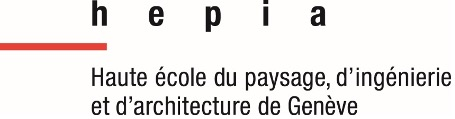
\includegraphics[height=1.29cm]{template/images/title/hepia_logo}};
\begin{spacing}{0.96}

	\begin{center}
		{\sf \fontsize{14pt}{16.8pt}\textsc{\textbf{\Orientation}}}\\*[1.5cm]
	\end{center}

	%% CONTENT STARTS HERE
	\noindent{\sf\textbf{Descriptif:}}
	La lumière Cherenkov est un phénomène physique similaire à un boom supersonique dans
	le domaine électromagnétique. Lorsque des particules chargées entrent dans notre atmosphère à
	la vitesse de la lumière, elles intéragissent avec les particules de celle-ci. 
	Ceci commence une réaction en chaîne produisant une pluie de rayonnements électromagnétiques
	et/ou de particules élémentaires telles que des protons par exemple.

	L'UNIGE travaille sur différents télescopes étudiant ce phénomène et souhaite améliorer
	la détection d'évènements intéressants physiquement pour réduire la quantité de données à stocker, transmettre et traiter.
	Pour cela, il est imaginé d'ajouter une étape de pré-traitement pour chaque pixel d'une caméra d'un télescope pour y filtrer
	le bruit des capteurs et effectuer une estimation calorifique du nombre de photons détectés.
	
	L'étape de pré-traitement utilisera le modèle de machine learning le plus capable à discerner 
	la ou les impulsions de photons à partir de la sortie analogique du capteur.

	\noindent{\sf\textbf{Travail demandé:}}
	Le travail demandé consiste à :
	\begin{itemize}
		\item Établir une série de tests et de métriques permettant de comparer différents modèles.
		\item Tester différents modèles de réseau de neurones (CNN/RNN/KAN).
		\item Intégrer l'étape de pré-traitement dans le pipeline du logiciel de classification de pluies Cherenkov : CTLearn.
		\item Exploration de l'utilisation du pré-traitement pour améliorer les performances de la stéréoscopie de CTLearn.
	\end{itemize}

	%% CONTENT ENDS HERE
	\vfill

	\begin{center}
		{\sf
			%%%%%%%%%%%%%%%%%%%%%%%%%%%%%%%%%%%%%%%%%%%%%%%%%%%%%%%%%%%%%%%%%%%%%%%%%%%%%%%%
			%%%%%%%%%%%%%%%%%%%%%%%%%% DO NOT MODIFY THE TABLE BELOW %%%%%%%%%%%%%%%%%%%%%%%
			%%%%%%%%%%%%%%%%%%%%%%%%%%%%%%%%%%%%%%%%%%%%%%%%%%%%%%%%%%%%%%%%%%%%%%%%%%%%%%%%
			\begin{tabular*}{16cm}{p{7.58cm} p{7.58cm}}
				\small Candidat-e:					&	\small Professeur-e(s) responsable(s):\\*[10pt]
				\small\textbf{\textsc{\Author}}		&	\small\textbf{\textsc{\Professor}}\\*[10pt]
				\footnotesize  Filière d’études : ISC	&	\footnotesize  \textbf{En collaboration avec:} UNIGE\\*[10pt]
				\footnotesize  {} & \footnotesize  Travail de bachelor soumis à une convention de stage en entreprise: \Convention\\*[20pt]
				\footnotesize  {} & \footnotesize  Travail soumis à un contrat de confidentialité: \Confidentiel\\*[10pt]
			\end{tabular*}\\*[0.5cm]
		}
	\end{center}
\end{spacing}